% author Dinupa Nawarathne
% email dinupa3@gmail.com
% date 10-11-2022

\documentclass[12pt, xcolor={dvipsnames}, aspectratio = 169]{beamer}

%
% packages
%
\usepackage{graphicx}
\usepackage{amsmath}
\usepackage{hyperref}
\usepackage[absolute,overlay]{textpos}
\usepackage{mathrsfs}
\usepackage[font=tiny]{caption}

%
% customization
%
\mode<presentation>
{
% custom colors
\definecolor{nmsured}{RGB}{137,18,22}
% custom fonts
\usefonttheme{serif}
\setbeamercolor{title}{bg=White,fg=nmsured}
\setbeamercolor{frametitle}{bg=White,fg=nmsured}
\setbeamercolor{section number projected}{bg=nmsured,fg=White}
\setbeamercolor{subsection number projected}{bg=nmsured,fg=White}
\setbeamertemplate{items}{\color{nmsured}$\blacksquare$}
\setbeamertemplate{section in toc}[square]
\setbeamertemplate{subsection in toc}[square]
\setbeamertemplate{footline}[frame number]
\setbeamertemplate{caption}[numbered]
\setbeamerfont{footnote}{size=\tiny}
\setbeamercovered{invisible}
}

%
% title, author, date
%
\title{Vertex Tagging: Sanity Check}

\author{Dinupa}

\date{NMSU Update
\\ October 18, 2022 }

\begin{document}

% make title page
\begin{frame}
    \maketitle
\end{frame}

% slides 2
\begin{frame}[fragile]{Receiver Operating Characteristic (ROC) Curve}

\begin{textblock}{7.0}(0.5, 2.0)
\begin{itemize}

    \item ROC curves typically feature true positive rate on the Y axis, and false positive rate on the X axis. This means that the top left corner of the plot is the “ideal” point - a false positive rate of zero, and a true positive rate of one. This is not very realistic, but it does mean that a larger area under the curve (AUC) is usually better.

\end{itemize}
\end{textblock}

\begin{textblock}{7.0}(8.0, 2.0)
\begin{figure}
    \centering
    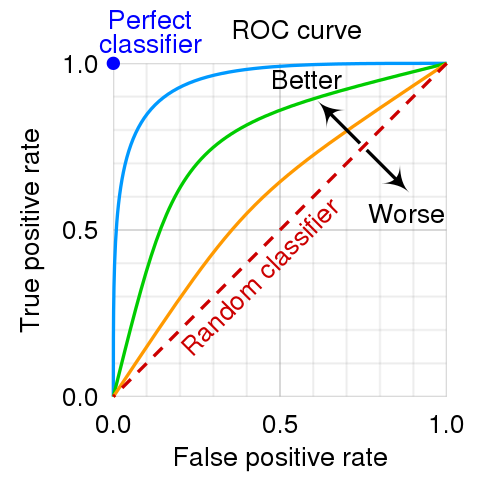
\includegraphics[width=7.0cm]{../imgs/Roc_curve.png}
\end{figure}
\end{textblock}

\end{frame}


% slide 3
\begin{frame}{Confusion Matrix}

\begin{textblock}{7.0}(0.5, 2.0)
\begin{itemize}
    \item Confusion matrix evaluate the accuracy of a classification.
    
    \item By definition a confusion matrix $C$ is such that $C_{ij}$ is equal to the number of observations known to be in group $i$ and predicted to be in group $j$.
    
    \item Thus in binary classification, the count of true negatives is $C_{00}$, false negatives is $C_{10}$, true positives is $C_{11}$ and false positives is $C_{01}$.
\end{itemize}
\end{textblock}

\begin{textblock}{7.0}(8.0, 2.0)
\begin{figure}
    \centering
    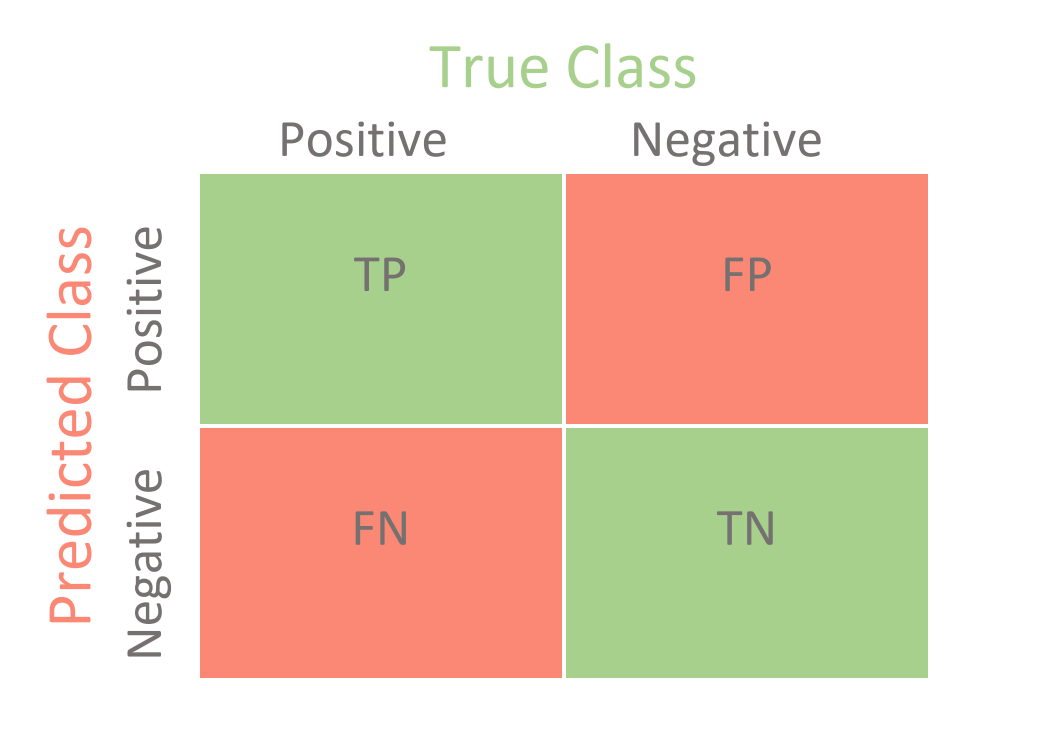
\includegraphics[width=7.0cm]{../imgs/con-mat.png}
\end{figure}
\end{textblock}

\end{frame}

% slide 4
\begin{frame}[fragile]
\begin{textblock}{14.0}(0.5, 0.5)

\begin{itemize}

    \item Labels;
    \begin{small}
    \begin{verbatim}
        position      | label      | int
    ------------------------------------
    -800. < z < -500. | collimeter | 0
    -500. < z < -305. | air1       | 1
    -305. < z < -295. | target     | 2
    -295. < z < 0.    | air2       | 3
    0. < z < 300.     | beam dump  | 4
    \end{verbatim}
    \end{small}
    \item Hot encoding;
    \begin{small}
    \begin{verbatim}
               | collimeter |air1    | target | air2   | beam dump
    --------------------------------------------------------------
    collimeter | 1          | 0      | 0      | 0      | 0
    air1       | 0          | 1      | 0      | 0      | 0
    target     | 0          | 0      | 1      | 0      | 0
    air2       | 0          | 0      | 0      | 1      | 0
    beam dump  | 0          | 0      | 0      | 0      | 1
    \end{verbatim}
    \end{small}
\end{itemize}

\end{textblock}
\end{frame}

\begin{frame}{ROC Curve and Confusion Matrix}

\begin{textblock}{7.0}(0.5, 2.0)
\begin{figure}
    \centering
    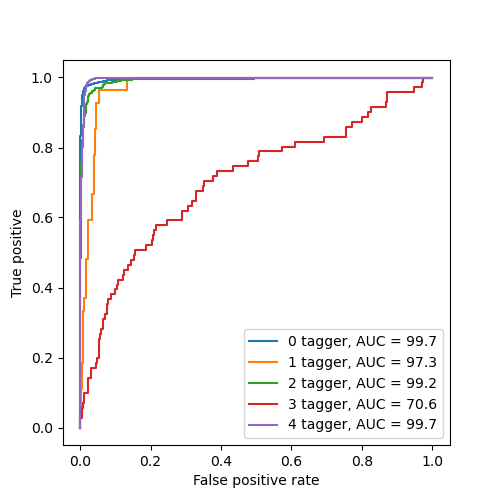
\includegraphics[width=7.0cm]{../imgs/roc-curve.png}
\end{figure}
\end{textblock}

\begin{textblock}{7.0}(8.0, 2.0)
\begin{figure}
    \centering
    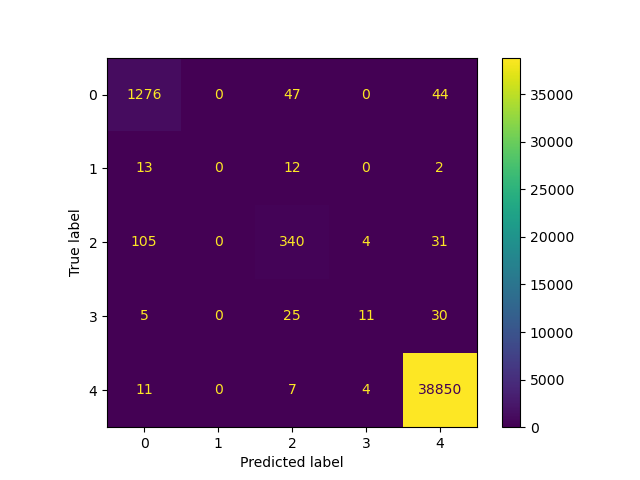
\includegraphics[width=7.0cm]{../imgs/cls-cm.png}
\end{figure}
\end{textblock}

\end{frame}

\begin{frame}{Loss}

\begin{textblock}{7.0}(0.5, 1.0)
    \begin{figure}
        \centering
        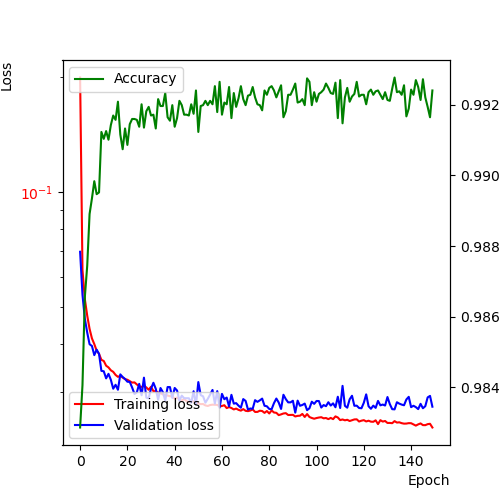
\includegraphics[width=7.0cm]{../imgs/cls-loss.png}
    \end{figure}
\end{textblock}

\begin{textblock}{7.0}(8.0, 1.0)
    \begin{figure}
        \centering
        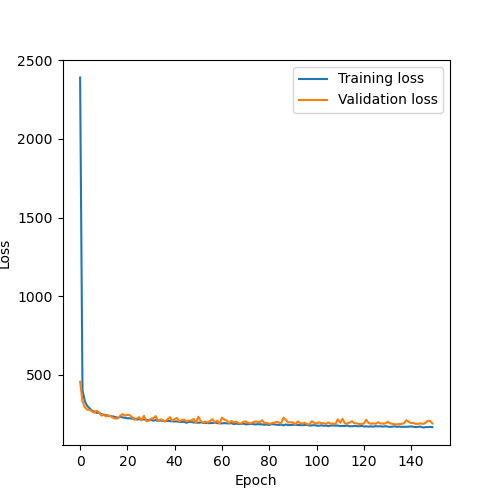
\includegraphics[width=7.0cm]{../imgs/reg-loss.png}
    \end{figure}
\end{textblock}

\end{frame}


% slide 5
\begin{frame}[fragile]{Tagging Task}
    \begin{textblock}{8.0}(0.2, 1.0)
        \begin{figure}
            \centering
            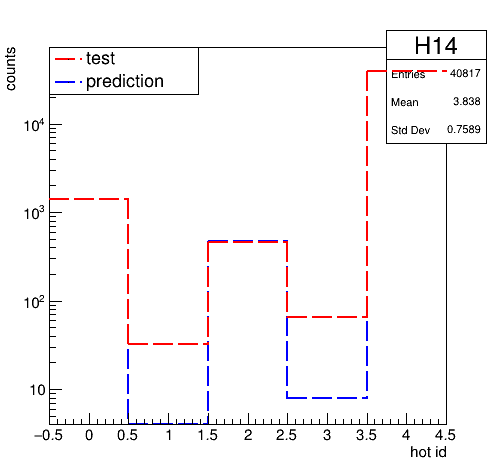
\includegraphics[width=8.0cm]{../imgs/hot_id.png}
        \end{figure}
    \end{textblock}
    
    \begin{textblock}{7.0}(8.0, 2.0)
    
    \begin{itemize}
        \item Classification layer almost predict bins except for bin with \verb|hot_id = 1, 3|, with 
        \verb|Accuracy for the test set: 0.9931|
    \end{itemize}
    
    \end{textblock}
    
\end{frame}


% slide 6
\begin{frame}

\begin{textblock}{14.0}(0.2, 0.2)
    \begin{figure}
        \centering
        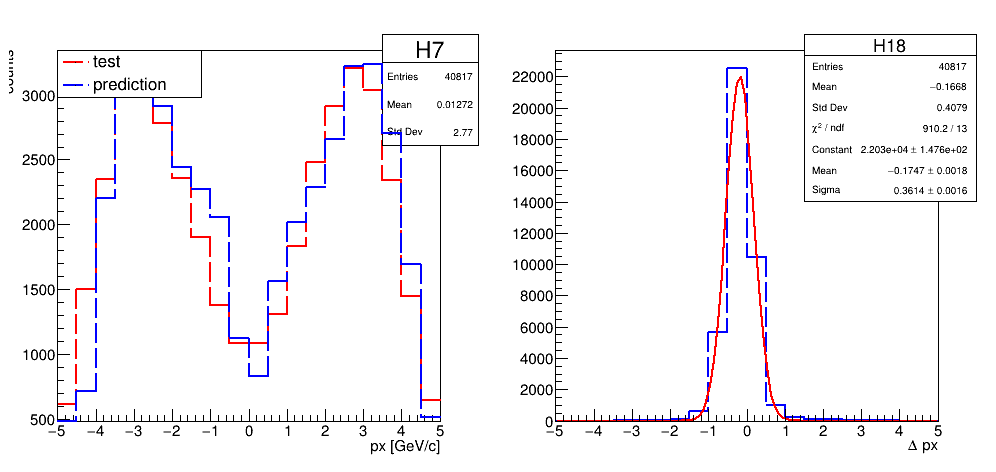
\includegraphics[width=14.0cm]{../imgs/vpx.png}
    \end{figure}
\end{textblock}

\end{frame}

\begin{frame}

\begin{textblock}{14.0}(0.2, 0.2)
    \begin{figure}
        \centering
        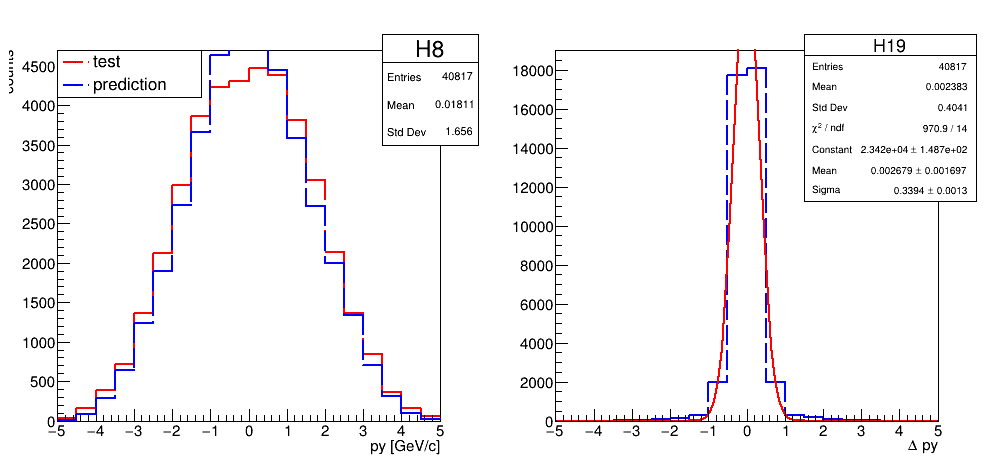
\includegraphics[width=14.0cm]{../imgs/vpy.png}
    \end{figure}
\end{textblock}

\end{frame}

% slide 7
\begin{frame}

\begin{textblock}{14.0}(0.2, 0.2)
    \begin{figure}
        \centering
        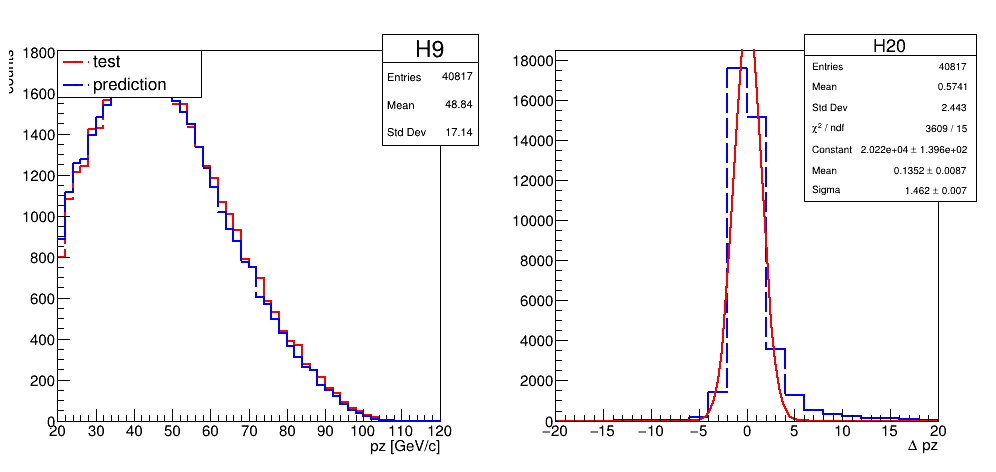
\includegraphics[width=14.0cm]{../imgs/vpz.png}
    \end{figure}
\end{textblock}

\end{frame}


% slide 8
\begin{frame}

\begin{textblock}{14.0}(0.2, 0.2)
    \begin{figure}
        \centering
        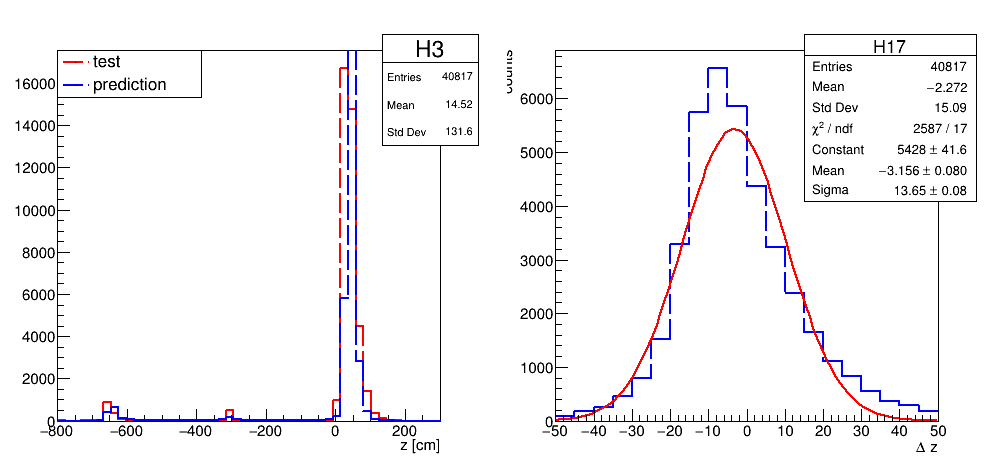
\includegraphics[width=14.0cm]{../imgs/vtz.png}
    \end{figure}
\end{textblock}

\end{frame}

\begin{frame}

\begin{textblock}{10.0}(0.2, 0.2)

\begin{itemize}

    \item Legacy method;

\end{itemize}

    \begin{figure}
        \centering
        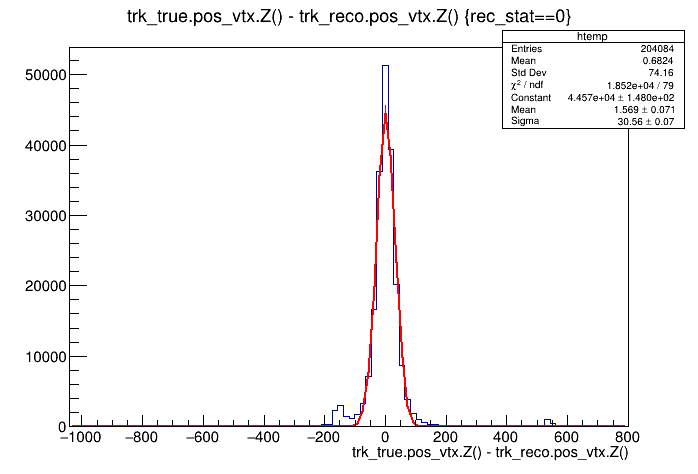
\includegraphics[width=10.0cm]{../imgs/c1.png}
    \end{figure}
\end{textblock}

\end{frame}

% slide 9
\begin{frame}

\begin{textblock}{14.0}(0.2, 0.2)
    \begin{figure}
        \centering
        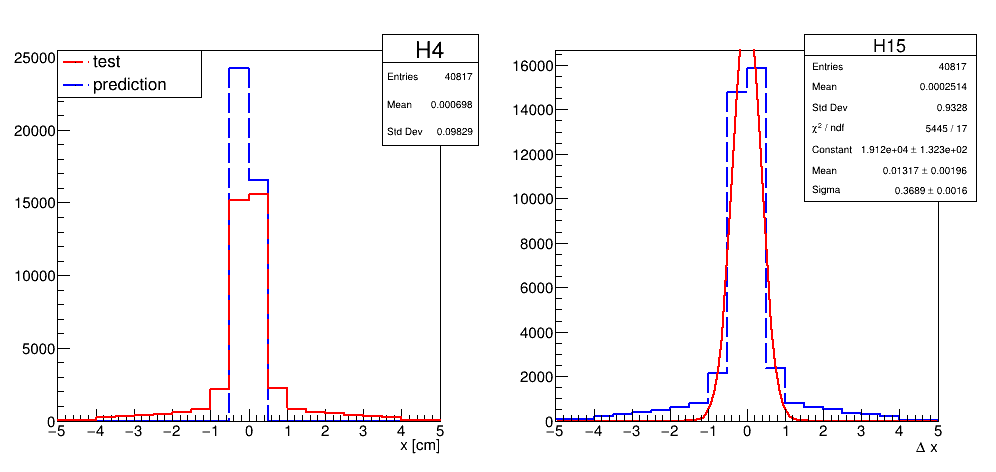
\includegraphics[width=14.0cm]{../imgs/vtx.png}
    \end{figure}
\end{textblock}

\end{frame}

\begin{frame}

\begin{textblock}{14.0}(0.2, 0.2)
    \begin{figure}
        \centering
        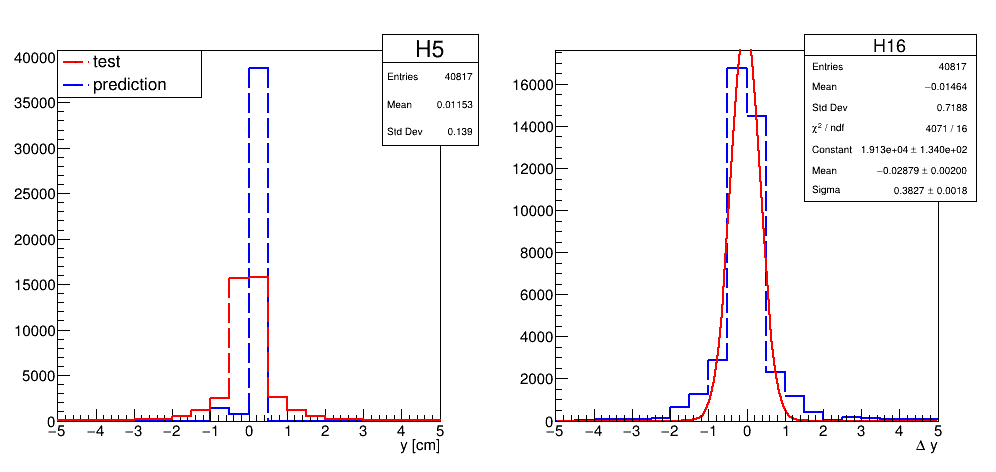
\includegraphics[width=14.0cm]{../imgs/vty.png}
    \end{figure}
\end{textblock}

\end{frame}

\begin{frame}{Preparation for Beam Time}

\begin{textblock}{14.0}(0.5, 2.0)

\begin{itemize}

\item Forhad and I plan to test the spare modules and make a inventory.

\item Optimising hodoscope efficiencies.

\begin{itemize}
    \item We have the software (Thanks to Forhad)
    \item Online monitoring ?
\end{itemize}

\end{itemize}

\end{textblock}

\end{frame}

\end{document}